\documentclass[11pt,technote,twocolumn]{IEEEtran}
\usepackage[utf8]{inputenc}
\usepackage{fullpage}
\usepackage{graphicx}
\usepackage{caption}
\usepackage{amsfonts}
\usepackage{amsmath}
\usepackage{biblatex}
\usepackage{array}
\usepackage[affil-it]{authblk}
\usepackage{fancyhdr}

\addbibresource{bibliography.bib}

\title{Using Speech Recognition and Social Media to Diagnose Mental Illness}

\author{\IEEEauthorblockN{Lynne Diep}\\
\IEEEauthorblockA{\textit{Computer Science Department, Jack Baskin School of Engineering} \\
\textit{University of California, Santa Cruz}\\
Santa Cruz, California \\
lytdiep@ucsc.edu}
}

\begin{document}

\maketitle

\section*{Abstract}
{\bf Using artificial intelligence in the medical field is no shock, but what if we use these same methods in diagnosing mental illness? Here we will discuss the incorporation of artificial intelligence in a psychological setting. Algorithms dealing with speech recognition and image comparisons are able to identify key words or representation of a patient dealing with mental illness. Computer assisted online social therapy allows users to speak anonymously as well. Of course mental illness does not have one single manifestation, so it is vital to develop algorithms which can represent different forms of indication. The results of this research will provide more insight on better determining mental illness through social media and the internet, and giving psychiatrists concrete evidence in their diagnosis.}
\footnote{Artificial Intelligence Conference} \footnote{https://conferences.oreilly.com/artificial-intelligence/ai-ca}
\footnote{Hannun A., Case C., and Caspter J.Deep Speech: Scaling up end-to-end speech recognition. Baidu Research – Silicon Valley AI Lab.}
\footnote{Garimella V., Alfayad A., Weber I. Social Media Image Analysis for Public Health. CHI '16 Proceedings of the 2016 CHI Conference on Human Factors in Computing Systems.}
\section{Introduction}
Artificial intelligence has been apparent since the creation of Greek mythology, but did not have significant development until the 1950s when scientists of all spectrum consider the creation of an artificial brain. Additionally, Alan Turing created the famous ``Turing Test" which indicated a computer was ``thinking" if the conversation between the computer and user was indistinguishable from an exchange between two human beings. Ultimately, the birth of AI was at the Darthmouth Conference in 1956 where AI received its meaning, calling, and support.
\par
As promising as the success of AI sounds, there are critiques of this extraordinary subject which led to financial setbacks which are known as the ``AI Winter". Despite these obstacles, AI found its footing in the 1990s when researchers developed algorithms which are still in use today. Data mining, speech recognition, logistics, medical diagnosis, and more are all branches from this AI tree, and have a significant impact in the technology industry. As society continues to expand, more technological advances are anticipated and AI will undoubtedly adapt to these adjustments.

\section{AI in the Medical World}
In the medical field, one of its main goals is to deliver effective treatment to patients, and to provide exact diagnosis. To have a computer to administer medical diagnosis, there must be several requirements which need to be met for the algorithm to ensue justifiable analysis. 
The computer must perform well, with the ability to appropriately deal with missing data and noisy data (errors in data). Ideal requisites of the computer must also have the ability to explain decisions and reduce the number of tests necessary to obtain reliable diagnosis. \cite{Kononenko:2001:MLM:2306296.2306356}
\par
For an algorithm to have good performance, it must be able to drive specific instruction from a cluster of data. With medical records, it is inevitable that data will be missing and will contain incorrect information so it is needed for algorithms to handle these factors. Having a computer being able to diagnose patients does not mean that a physician's job is replaced, it is only there to fill in the gaps the physician might have missed. The machine must be able to pass on its information in a way which the physician can understand and allow them to conduct the next step. There are countless amounts of patients' data and having to sort through them is time consuming, so the ideal algorithm would be able to diagnose a patient with the least amount of recent data as well.
\par
\begin{table*}[t]
\centering
 \begin{tabular}{||c c c c c ||} 
 \hline
 Classifier & Performance & Transparency & Explanation & Reduction \\ [0.5ex] 
 \hline\hline
 Assistant-R & Good & Very good & Good & Good \\ 
 \hline
 Assistant-I & Good & Very good & Good & Good \\
 \hline
 Naive Bayes & Very good & Good & Very good & No\\
 \hline
 Semi-naive Bayes & Very good & Good & Very good & No\\ 
 \hline
 Backpropagation & Very good & Poor & Poor & No 
 \\
 \hline
 $k$-NN & Very good & Poor & Acceptable & No \\ [1ex]
 \hline
\end{tabular}
\caption*{Table 1: Classifers and their performance}
\end{table*}
\\Currently, there are state-of-the-art algorithms used in the medical field, and Igor Kononenko has compared them with the requirements a ``good" algorithm should have as shown in Table 1 above.

A brief summary of some of the classifiers will be explained.

\subsection{Naive and Semi-Naive Bayesian Classifiers}
These classifiers are of interests to physicians because it consists an agenda of condition properties, which is given by
\begin{align*}\tag{1}
    -log_2P(C|V_1, \ldots, V_n) = -log_2P(C)
    \\
    \sum_{i}(-log_2P(C) + log_2P(C|V_i))
\end{align*}
In (1), the Naive Bayesian represents the information needed to find if an instance belongs to class $C$. For the Semi-Naive Bayesian, the set up is identical excluding when value pairs occur. When this happens, the joined values are used rather than the simple attribute values. The data gathered from this algorithm can then be summed up in a table for confirmation to accept or reject the decision. Each attribute present has a contrasting strength which can influence the classifier. Physicians use the Bayesian Classifiers because they believe the machine goes through the same thinking process as they do.
\subsection{Assistant and ReliefF}
The Assistant-R and Assistant-I are expansions of the Assistant algorithm which is top-down induction of decision trees. The differences between these two extensions is that Assistant-I uses informativity, while Assistant-R uses the algorithm ReliefF. When dealing with multi class problems, the ReliefF algorithm selects the nearest neighbor samples from each of the samples in different categories. Randomly select a sample $x$ from the training sample, then to find out $k$ nearest neighbor samples from the kind of sample $x$, and randomly find out $k$ non similar nearest neighbor samples from neighbors of different classes. To adjust a feature weighting vector to give more weight to features by comparing within-class distance and between-class distance from neighbor samples. Repeat the above procedure on each feature dimension, finally get the weight value of each feature.\cite{7729190} The overall algorithm is:
{\small{
\begin{align*} \tag{2}
    W_{\mathrm{f}}^{i+1}= W_{f}^{i}+ \sum\limits_{{c}\neq class(\mathrm{x})}\frac{\frac{p(\mathrm{x})}{1-p(\text{class}(\mathrm{x}))}\sum\limits_{j=1}^{k} diff_{f}(\mathrm{x},\mathrm{M}_{j}(\mathrm{x}))}{m^{\ast}k} 
    \\
    - \sum\limits_{j=1}^{k}diff_{f}(\mathrm{x},\mathrm{H}_{j}(\mathrm{x}))/(\mathrm{m}^{\ast}\mathrm{k})
\end{align*}}}%
As seen in Figure 1, the Assistant algorithms received positive feedback regarding the requirements needed for an algorithm to diagnose medical illness. 
\subsection{Using These Methods for Mental Illness}
Similar to medical conditions, mental illnesses have symptoms which can help psychiatrists diagnose patients. If the algorithms used in the medical field can help physicians in a significant way, then the use of these algorithms in the psychiatric field can surely have the same effect.
\par
For example, by using the Bayesian Classifiers psychiatrists can use the data gathered and make a firm decision; similar reasoning with the Assistant and ReliefF algorithms as well. Physicians believe the machine goes through the same contemplative process as they do, so the machine should be able to do the same for psychiatrists.
\section{Examining Speech and Actions for Mental Illness}
Unlike medical diagnosis, there are no laboratory tests to determine mental illness. Doctors may use assorted test to find out if there is something which is causing the patients symptoms, but will most likely result in seeing a psychiatrist or a mental health professional to receive the appropriate care. Mental health professionals conduct tests regarding the patient's speech, behavior, and actions. After the tests are run, the specialist decides if the results correlate with any mental illnesses.
\par
Analyzing a patient's speech is one of the most common tests in diagnosing mental health. Disorganized speech where the individual has a hard time focusing on one subject or when their dialogue is incomprehensible is an indication of illness depending on the severity of it. By all means, it is important to consider disorganized speech is a common circumstance, and should not be the only element when diagnosing mental health.
\par
The next form of indication is an individual's behavior. When an individual's behavior is causing infliction on their self or others around them, it is a sign of ill mental health. Additionally when the individual partakes in not socially sanctioned activities, such as substance abuse, getting tattoos and piercings, and more especially if they had no interest in them before. Ultimately, if the person's behavior is affecting them in a negative way like their academics are falling or their personal relationships are crumbling, then it is best to check their mental health.
\par
There are more factors in determining a patients mental health, and it is important to consider that every case is different. For algorithms to successfully perform in the psychological field, they must be able to execute several variables to examine the different forms on mental health. 
\subsection{How AI Can Come Into Play}
Since the birth of AI, AI has evolved tremendously since the birth of it, for example, Google's Assistant and Amazon's Alexa uses the power of speech recognition to perform daily tasks. Recently, Google announced its AI is watching YouTube videos to analyze human behavior. As mentioned before, AI in the medical field is nothing unfamiliar and it is proven to make a significant impact for physicians. Using speech recognition and behavior analysis is exactly what psychiatrists test in patients and by integrating these techniques and modifying them to fit psychiatrists needs, there is no negative aspect in at least trying this approach. 
\section{Speech Recognition}
Speech recognition is still a fairly new concept which is gaining popularity as new technologies are incorporating speech recognition into its products. Apple's Siri allows users to talk to an intelligent personal assistant which has a mind of its own. Anyone with the capability to speak can request Siri to search movie times, the current weather forecast, or what song is currently playing all by talking to their device like how they do with human beings. Additionally devices like Siri are able to correct the user when they speak incoherent sentences. If machines like Siri and other home devices are able to support users for secretarial tasks, then the use of speech recognition has the power to support those in the professional field.
\subsection{Recurrent Neural Network (RNN)}
The core of a speech recognition system is a RNN trained to ingest speech spectrograms and generate English text transcriptions. Let a single utterance $x$ and label $y$ be sampled from a training set 
\begin{math}
X = \{(x(1), y(1)),(x(2), y(2)),\ldots\}
\end{math}
Each utterance, $x^{(i)}$, is a time-series of length $T^{(i)}$ where every time-slice is a vector of audio features, $x_t^{(i)}$, $t=1$, $\dots$, $T^{(i)}$. Spectrograms will act as the features, so $x_{t,p}^{(i)}$ denotes the power of the $p$’th frequency bin in the audio frame at time $t$. The goal of our RNN is to convert an input sequence $x$ into a sequence of character probabilities for the transcription $y$, with $\^{y}_t = P(c_t|x)$, where $c_t$ $\in$ \{a,b,c, \ldots, z,space, apostrophe, blank\}. 
\par
\begin{table*}[t]
\centering
\begin{tabular}{|l|l|}
\hline
RNN Output                                   & Decoded Transcription                        \\ \hline
what is the weather like in bostin right now & what is the weather like in boston right now \\
prime miniter                                & prime minister                               \\
arther n tikets for the game                 & are there any tickets for the game           \\ \hline
\end{tabular}
\caption*{Table 2: RNN Transcription}
\end{table*}
The RNN is composed of five layers of hidden units, where the first three layers are not recurrent. For the first layer, the output relies on the spectrogram frame $x_t$ for each time $t$. The leftover layers will rely on independent data for each step. The first three layers will operate through this formula:
\begin{equation}\tag{3}
    h_t^{(l)} = g(W^{(l)}h_t^{(l-1)}+b^{(l)})
\end{equation}
The fourth layer is a bi-directional recurrent layer, and has two sets of hidden units which are a set with forward recurrence $h^{(f)}$, and a set with backward recurrence $h^{(b)}$ which is expressed as:
\begin{equation}\tag{4}
    h_t^{(f)} = g(W^{(4)}h_t^{(3)} + W_r^{(f)}h_{t-1}^{(f)} + b^{(4)})
\end{equation}
\begin{equation*}
     h_t^{(b)} = g(W^{(4)}h_t^{(3)} + W_r^{(b)}h_{t+1}^{(b)} + b^{(4)})
\end{equation*}
The fifth layer is non-recurrent and takes the backward and forward units as input $h_5^{(5)} = g(W^{(5)}h_t^{(4)} + b^{(5)})$ where $h_t^{(4)} = h_t^{(f)} + h_t^{(b)}$. The function (5):
\begin{equation}\tag{5}
    h_{t,k}^{(6)} = \^{y}_{t,l} \equiv P(c_t = k|x) = \frac{exp(W_k^{(6)}h_t^{(5)}+b_k^{(6)})}{\sum_j exp(W_j^{(6)}h_t^{(5)}+b_j^{(6)})}
\end{equation}
is the output layer which returns the predicted character probabilities for each time $t$ and character $k$. \cite{DBLP:journals/corr/HannunCCCDEPSSCN14}

\par
Overall the RNN algorithm can learn to generate readable character-level transcriptions. The results of this algorithm is satisfactory, as it transcribes the input into a readable, define output. In Table 2 above, an example of transcription is given.

As seen in the Decoded Transcription in the table above, the results are coherent and allow the user to fully understand what the RNN output is.
\subsection{Application}
The opportunity to use this algorithm in the psychiatric field would be valuable. To individuals who jumble up their words or are unable to speak proper sentences, RNN would be able to decode their conversations in hopes of mental health professionals gaining a better understanding of their situation. In fact Medium reports that IBM Research is using transcripts and audio from psychiatric interviews, coupled with machine learning techniques, to find patterns in speech to help clinicians accurately predict and monitor psychosis, schizophrenia, mania, and depression. Today, it only takes them about 300 words to help clinicians predict the probability of psychosis in a user. So AI is a revolutionizing tool in the mental health field and with this approach, there would be more evidence to support an individual's diagnosis.
\par
However, the use of speech recognition will only work if the individual is willing to speak. If they do not feel comfortable speaking out loud, then this method is ineffective. There are techniques which can go around this matter, such as computer assisted therapy, text analysis, and image analysis on social media.
\section{Textual Analysis on Social Media}
In this technological age, people of all ages have or interacted with social media. More than 1.8 billion images are shared each day through media outlets, and many showcase individuals' daily lives. Due to the popularity of social media there is an abundance of data, hence, the use of data mining and social media privacy are extensive issues among users. However, the use of image analysis can tell more about an individual than one might expect. Through the progress of deep learning, the prospect of understanding objects through images and generating textual descriptions has become reality.
\par
\begin{figure*}[t]
    \centering
    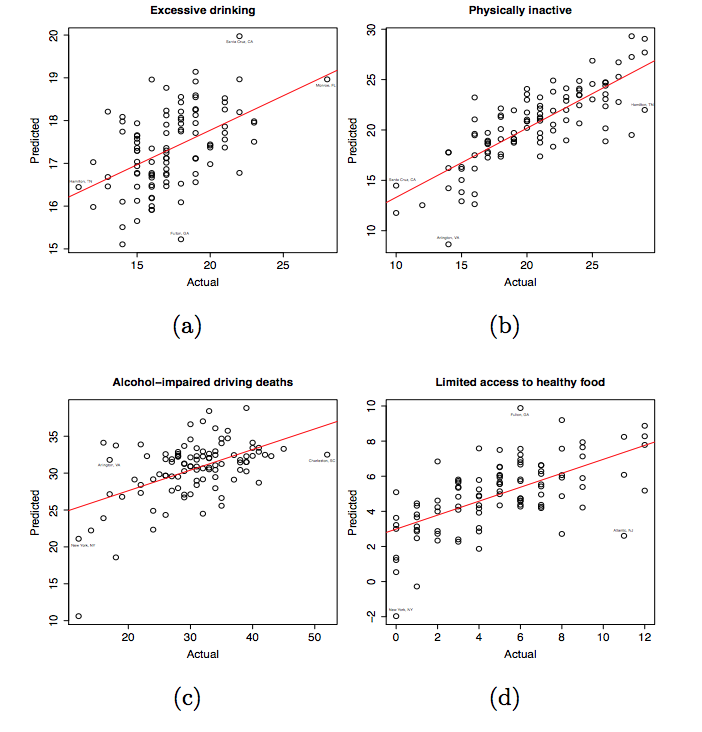
\includegraphics[width=330px]{Graph}
    \caption{Predicted vs.\hspace{1mm}actual health statistics value using (a) Tags for predicting excessive drinking, (b) User-provided tags + demographics for predicting physically inactive, (c) User-provided tags for predicting alcohol-impaired driving deaths, and (d) User-provided tags for predicting limiting access to healthy food. }
\end{figure*}
Social media makes it easier to let others know what an individual is doing, where they are, and who they are with by tagging the respective nouns on their images. Additionally, users can caption their image with a corresponding message. The message can indicate what the user is doing, how they are feeling with the use of emoticons, or any message that is on their mind. By analyzing the words used in captions and tags, psychologists can group key words which represent different forms of mental illness. For example, if an individual has posted images along with a caption that contain words from a predetermined set of terms describing depression, then the individual may have depression.

\subsection{Support Vector Machine (SVM)}
SVM is a part of machine learning and is used to analyze textual descriptions and classify them using predetermined set of terms. Linear binary SVMs are trained by finding a hyperplane defined by a normal vector $w$ with the maximal margin separating it from the positive and negative datapoints. Finding such a hyperplane is inherently a quadratic optimization problem given by the following objective function.\cite{Sadilek:2013:MIL:2433396.2433476}  
\begin{equation}\tag{6}
    \min\limits_{w} \frac{\lambda}{2} ||w||^2 + L(w,D),
\end{equation}
where $\lambda$ is a regularization parameter controlling model complexity, and $L(w, D)$ is the hinge-loss over all training data $D$ given by
\begin{equation}\tag{7}
    L(w,D) = \sum_i max(0,1 - y_{i}m^{T}x_{i}).
\end{equation}
Regarding word tokens, SVM uses all unigram, bigram, and trigram phrases; for example if the caption is ``I am sad", then the feature vector:
\begin{align*}
(I, \hspace{.7mm}am, \hspace{.7mm}sad, \hspace{.7mm}I \hspace{.7mm}am, \hspace{.7mm}am \hspace{.7mm}sad, \hspace{.7mm}I \hspace{.7mm}am \hspace{.7mm}sad)
\end{align*}
represents the caption. These phrases will be analyzed and specific weights will be added to them determine the significance. For instance, if the word ``sad" has been a common statement for those suffering from depression then when an individual uses ``sad" in there conversation a relatively large weight will be added to this feature. As each word in the patient's phrase is analyzed and assigned weights, the total weight is a part of a determining factor in a psychiatrist's diagnosis.
\par
Along with the use of SVM, decision trees are utilized as well. The decision tree represents a set of questions which are answered by the individual to determine their health.  Features are evaluated in terms of information gain with respect to the labels and the best candidates are subsequently selected for each inner node of the tree. \cite{Sadilek:2013:MIL:2433396.2433476}
\subsection{Application}

Using methods like SVM, psychiatrists and other professionals are able to examine individuals through social media. Additionally professionals are able to research large communities, such as counties, through the convenience of geo-tagging on social media platforms like Instagram. The correlation between image analysis and actual health statistics is not inaccurate either, so it does provide stable evidence when diagnosing an individual as seen in Figure 1. Monitoring a user's alcohol intake, substance use, and physical activity through their social media allows doctors to see their progression of these activities. If these actions show an increase or there is relapse, then this is an indication of possible incidents of mental health and shows evidence for professionals to move forward with the proper care. 

\section{Image Analysis on Social Media}
Social media applications, such as Instagram, Facebook, and Twitter give users the opportunity to post pictures of their personal lives showcasing their activities and daily occurrences. Analyzing image content can give a further glimpse into the posters' lives and determine if their representation of themselves online is contributing to their unhealthy lifestyle. In order to pinpoint images and correlate them into significant data, there has to be specific ``image interests" to look out for. For example if the user in question is examined for alcoholic behavior, then the ``image interest" would be bottles of alcoholic beverages. Then the algorithm used would analyze the user's images and pinpoint pictures containing the specified interest. Using this method in diagnosing mental illness is efficient due to the popularity of social media and its users willing to present more of their lives to the public than to a therapist.
\par
There are many features in an image to analyze; color, texture, shape and Scale Invariant Feature Transform (SIFT) are prospects to consider when considering pictures in question.
\subsection{Color}
Regarding the color of an image, there are two color-based features of interest color histogram and color moments, which capture the distribution of different colors in the images.\cite{5202725} An image's color can actually express a user's mental state. For example, Instagram gives users the option to put a filter on their photos before publishing them. A filter can either brighten up the photo, or give the photo a dark, ominous feeling depending on their choice of editing. In a study of 166 people, where researchers identified those who have been diagnosed with depression and those who had not, results stated that those who have been diagnosed are less likely to filter their photos than those people who are not diagnosed with depression. ``Inkwell” — a filter which turns photos black-and-white — was the most popular filter used by depressed people, whose photos were more likely than their nondepressed peers to contain a face. By comparison, the ``Valencia,” was popular among more mentally healthy users.\cite{de2013predicting}
\subsection{Texture}
The texture of an image gives information about the spatial arrangement of color or intensities in an image or selected region of an image. The two texture features which will be used for analysis are gray level co-occurrence matrix (GLCM), and a texture detector for arbitrary ``blobs” in images called phase symmetry.\cite{6879475} Phase symmetry is based on determining local symmetry and asymmetry across an image from phase information. Given an image, phase-based symmetry detector (PSD) maps a pixel, $p$, an orientation, $o$, and a scale, $n$, to a phase congruency value $PC_{no}(p)$ and a special phase, $\phi_{no}(p)$:
\begin{equation}\tag{8}
    PSD(p,n,o)=(PC_{no}(p)\phi_{no}(p))
\end{equation}
Here,
\begin{equation}\tag{9}
    PC_{no}(p)={{\rm sum} E(p)\over {\rm sum}A(p)+\varepsilon}={\sum\limits_{k,q}E_{n_{k}o_{q}}(p)\over \sum\limits_{k,q}A_{n_{k}o_{q}}(p)+\varepsilon}
\end{equation}
where sum$E(p)$ is the total energy when phases are congruent under all scales and orientations and phases are zero; sum$A(p)$ is the total amplitude when phases are congruent under all scales and orientations and phases are zero; $\varepsilon$ is a positive constant.\cite{5202725}
\subsection{Shape}
The shapes within the image is another key feature to examine. For example, a shape of a bottle or a shape of a syringe can easily be recognized if they were the focal point of an image. However in most cases, people do not intend to showcase these possessions and will do their best to hide them. With the shape feature in image analysis, these items of interest can be brought to attention which would of otherwise been overlooked by human perception.
\par
Images are often characterized by central themes or concepts. To extract such features, the use of two shape features are radial symmetry and phase congruency. The radial symmetry feature is based on the idea of detecting points of interest in an image. Phase congruency is an illumination and contrast invariant measure of feature significance. For a given image, phase congruency $PC(x)$ at some location $x$ is expressed as the summation over orientation $o$ and scale $n$:
\begin{equation}\tag{10}
PC(x)={\sum\limits_{o}\sum\limits_{n}W_{o}(x)\left\lfloor A_{no}(x)\Delta\Phi_{no}(x)-T_{o}\right\rfloor \over \sum\limits_{o}\sum\limits_{n}A_{no}(x)+\varepsilon}
\end{equation}
where $A_n$ represents the amplitude of the nth component (of the image) in the Fourier series expansion, $W_o(x)$ is the convolution of the given image with an even / odd filter, $\varepsilon$ is added for cases of small Fourier amplitudes, To is a compensating measure for the influence of noise and $\Delta\Phi_{no}(x)$ is a sensitive phase deviation.\cite{5202725}
\subsection{SIFT}
SIFT is a  content-based image feature which detects stable keypoint locations in scale space of an image. It computes the following function from the difference of two nearby scales separated by a constant multiplicative factor $\kappa$:
\begin{equation*}
D(x, y,\sigma) = (G(x, y, \kappa\sigma)-G(x, y,\sigma))\ast I(x, y)\cr 

= L(x, y, \kappa\sigma)-L(x, y,\sigma)      \hfill(11)
\end{equation*}
\\
\\
where $L(x, y,\sigma)$ is the scale space of image $I(x,y)$ and is produced from the convolution of a variable-scale Gaussian having scale $(\sigma)$ with $I(x,y)$.\cite{5202725}
\subsection{Applications}
Using image analysis will provide significant evidence and data in diagnosing mental illness. Social media puts no boundaries on users and most individuals feel more comfortable to express themselves on this platform than they do in their typical lives. As brought up in 6.3, image analysis can uncover more information about a user than the human eye. The cliche, ``A picture is worth a thousand words" is relevant in this case and can potentially help those who are hesitant and unsure of how to approach treating their mental health.
\section{Computer Assisted Online Social Therapy}
Many individuals, especially those on the younger side, do not feel comfortable with confronting their matters head-on, and are more likely inclined to express themselves online through platforms like social media. Chat rooms where users can conceal their identity but still communicate with people with the same interests are common outlets as well. These outlets allow people to express themselves without feeling the pressure of being judged and ridiculed by their peers. Additionally, the person who the user is talking to is equipped with knowledge on how to advise them with their situation. Essentially, computer assisted online social therapy provides a safe space for users while giving the option of being anonymous and still receive the care and advice for treating their concerns.
\subsection{Automated Suggestions}
Although human-supported engagements is a key part in online therapy sessions, the move to automated suggestions is gaining traction. The first obvious advantage of automated suggestions over moderator suggestions is that they are not limited to times when moderators are available on the system and furthermore they can be delivered to the user in real-time. Automated suggestions also facilitate scaling the site to a larger user group. \cite{Alfonso} To determine how the machine interacts with the user, a combination of the post's sentiment, emotion scores, and keywords to determine its most relevant steps and actions.
\par
Here is a pseudocode of the algorithm:
\begin{enumerate}
    \item Upon submission of a post to the newsfeed, a call is made to IBM's Alchemy text analysis system. First, it provides a score for the post's sentiment, with score $= 0$ being neutral, $1 >$ score $> 0$ being positive, and score $0 >$ score $> −1$ being negative. Second, it provides a score between $0$ and $1$ for the emotions of Anger, Disgust, Fear, Joy, and Sadness. Third, it extracts the post's keywords.
    \item Our steps and actions have been partitioned into those which are suitable for positive posts, those which are suitable for negative posts and those which are suitable for either. We use this partitioning such that if a post is positive then a set of suggestion candidate steps/actions is reduced to those marked positive. Similarly for negative. If the post is neutral, then no such reduction is made.
    \item Our steps and actions have also been assigned measures for each of the five emotions mentioned in point 1; the higher the measure, the more relevant the item is for posts exhibiting that emotion. We also have extracted and stored the keywords for all of our steps and actions. Given this, each of the candidate steps/actions is assigned a score based on their semantic similarity with the post's keywords and congruence with the post's emotion measures.
    \item The step with the highest score is selected as is the action with the highest score. If more than one candidate emerges, at this stage one is randomly chosen.
\end{enumerate}
The keyword semantic similarity component is the most decisive factor in these calculations. Given that much of therapy content is specifically suited to only positive or negative states, the sentiment analysis component determines an important initial partitioning of therapy content where applicable. The emotion congruence component provides a balancing and adjudicating factor. First, it can distinguish therapy items which have the same semantic similarity score. Second, it can ``downgrade” therapy items with a relatively high semantic similarity score that are otherwise emotionally inappropriate relative to the post. \cite{Alfonso}
\subsection{Chatbots}
Chatbots are conversational agents which interacts with users on specific topics of interest with natural languages. Developed chatbots on the internet include Eliza, Claude, and ALICE. Regarding Eliza, it was the first chatbot to be developed and was designed to emulate a psychotherapist and had a knowledge base in this domain. Most chatbots consist of a dialog management module and a chatbot knowledge base, which can be thought of as a brain for the chatbot. The ``brain" contains information on how to respond to the user based on their input. The dialog management module controls the process of dialog between the computer and user, such as receiving and understanding user input and searching for the appropriate response based on the chatbot knowledge. In order to have the chatbot replies be relevant and impactful, the chatbot knowledge extraction is based on a rough set; it extracts structural and content features of different replies, and uses ensemble learning method in the decision-making stage. \cite{4663330}
\par
A rough set is built on the classification mechanism and regards classification as indiscernibility (equivalence) relations. Indiscernibility relations constitute division of the space. Rough set theory regards knowledge as the division of the data. Rough sets are popular in the AI field and used in knowledge acquisition, knowledge analysis, and decision analysis. Ensemble learning constructs multiple learners and combines the classification results of the learners to get the final results. This method can improve the generalization of learners and is popular in machine learning, data mining, and AI.
\subsection{Rough Set}
To determine how the chatbox will interact with the user, the use of a classification model based on a rough set will be used.An input online discussion forum $F$ contains discussion sections $s_1, \dots, s_k$. Each section consists of $u$ threads $t_1, \ldots, t_u$. Each thread $t$ is a sequence of replies $t = \{r_0, \dots, r_n\}$, where $r_0$ is the root message posted by the thread starter and $r_1$ is the $ith(i \geq 1)$ reply. Replies are classified into related replies (RR) and irrelated replies (IR). RR is defined as a direct reply to the root message and it is not correlated with the other replies in the thread. The others are called IR. By analyzing a certain number of replies, the feature set is obtained.\cite{4663330}
\par 
Here are the definitions of the classification model:
\begin{enumerate}
    \item An online forum reply classification system is a 4-tuplle $S = \{ U, R = C \cup D, V, f \rangle$, where $U$ is a set of replies. $R$ is a set of attributes, $c$ is a set of reply attributes, and $D$ denotes the decision attribute, whose value is the type of the replies. $V$ is the domain of the attributes. $f$ is an information function which denotes the attribute value of each $x$ in $U$.
    \item Indiscernibility relations in $U : P$ is a set of attributes, $P \subsetequal R$, object $X, Y \in U$, for each $a \in P$, if $f(X, a) = f(Y, a)$, we call $X$ and $Y$ have indiscernibility, that is $ind(P) = \{(X,Y) \in U^2, \forall a \in P(f(X,a) = f(Y,a))\}$ . Here $ind(P)$ is an indiscernibility relation. Then attribute set $P$ can be regarded as a knowledge name with equivalence relationship. So an online forum reply classification system can be regarded as a knowledge base system. When a reply is needed to be analyzed, we select the corresponding knowledge base rule according to $ind(P)$, and get the classification result.
\end{enumerate}
By analyzing the significant amount of replies, the following reply attribute set is defined:
\begin{equation} \tag{12}
    C = A_0 \cup A_1 \cup A_2 \cup A_3 \cup A_4 \cup A_5
\end{equation}
The meaning of these features are:
\begin{enumerate}
    \item $A_0$: Is this reply posted by the tread starter? 1 means yes, while 0 means no.
    \item $A_1$: Interval of replies between same author's previous and current reply.
    \item $A_2$: Quotation of the reply. No quotation is shown as 0. Quotation of root message is shown as 1. Quotation of other reply is shown as 2.
    \item $A_3$: Whether the reply has feature words which show it is not a relative reply? Define the following words: up, same questions, good reply, collecting, help, and so on.
    \item $A_4$: The number of reply words.
    \item $A_5$: The number of questions marks in this reply.
\end{enumerate}
By using the decision rules of data preprocessing, reduction of attributes, reduction of values, and obtaining logic rules, the results will tell the chatbox the appropriate reply to the user. \cite{4663330}
\subsection{Ensemble Learning}
For ensemble learning, the method of Bagging is used for the basis. Given a data set $L = \{(x_1,y_1), \ldots, (x_m,y_m)\}$, and a basic learner $h(x,L)$ to predict $y$. Now there is a sequence of data sets $\{L_k\}$, where each sequence is composed of $m$ independent observations which have the same distribution of $L$. The goal is to use $\{L_k\}$ to find a better learner than the learner from a single set of data.
\par
Here is the pseudocode of the Bagging algorithm:
\begin{flushleft}
Input: training set $S = \{(x_1,y_1), \ldots, (x_m,y_m)\}$, a weak learner.
\\
WeakLearn, the biggest round $T$ of training.
\\
\hspace{5mm} Output: an ensemble prediction model.
\\
\hspace{5mm} Step 1: Extract $m$ training subsets $S'$ from raw set $S$ using the method of bootstrap.
\\
\hspace{5mm} Step 2: Train weak learners on $S'$ and get the round $t$ hypothesis function $h_t$.
\\
\hspace{5mm} Step 3: If $t < T$, go to Step 1 and set $t=t+1$, else fo to Step 4.
\\
\hspace{5mm} Step 4: Combine multiple hypothesis $h_1,h_2, \ldots, h_r$ to get the final hypothesis function: $h_A (x) = sign(\sum h_1(x))$.
\\
\hspace{5mm} Step 5: The end.
\end{flushleft}
\par
The decision to use Bagging instead of Boosting is because in Bagging, bootstrap sample is used and the scale of the training sets is familiar with the original training sets. Boosting will not produce compelling data in this case because the selecting of the training set depends on the performance of the previous learner. So if the previous learner has been wrongly classified, then the training set will be selected on incorrect data and botch the process. Boosting can get superior classification results than Bagging; however, Boosting may lead to over fitting in handling some practical problems and get even worse results than a single learner. With this in mind, Bagging is the algorithm which will be used in this case. \cite{4663330}
\section{Prospects to Consider}
The current use of AI in the medical field works sufficiently, and there are no major complications which disrupt physicians' responsibilities and activities in serving society; however, in the case of AI in the psychiatric field, there are a few things to consider: mental health is different for every individual, individuals may have health disabilities which affect the way they talk and act, being unable to store each individuals' extensive data, and more within this scope.
\par
Regarding the different cases of mental health, it is important for the AI to treat each individual separately and not base diagnosis on controlled settings. The machine must be able to incorporate standard symptoms of an illness while taking note of the unique psychical and mental features of the patient. Additionally the algorithms used must be able to acknowledge multiple variables as there is no finite number of variables for each individual.
\par
Speech recognition and image/textual analysis are some of the tools used to diagnose both mental and physical health issues, but it is essential to acknowledge those with disabilities which hinder them from participating in these exams. Additionally, there are users who do not partake in social media activities or do not have access to online resources, so it is important to be cautious of people's accessibility. Obviously, it is already difficult to find methods in treating those with disabilities so the use of AI in this field will be challenging to overcome.
\par
Going back on the issue of data control, the machine must be able to hold a significant amount of statistics and information. This is a similar issue for AI in the medical field, and it is still a relevant concern to resolve.

\section{Conclusion}
AI has proven to become more powerful as time progresses, and utilizing its capabilities will definitely open new opportunities towards society. Regarding the use of AI in the psychiatric field, there are benefits of using these methods that are similar to AI in the medical field. 
\par
Speech recognition is a promising approach in diagnosing mental illness. RNN is able to translate an output to a decoded transcription which displays proper sentences easier to read and understand. As seen in Figure 2, the RNN algorithm allows doctors and professionals to get a better grasp of what the patient is trying to say. This is indeed helpful, especially if the patient has difficulty speaking in full and proper sentences. A setback in this method is that it does not work if the patient is unwillingly or unable to speak verbally, so obviously speech recognition would not work in this case.
\par
Textual analysis on social media is another approach which has potential in diagnosing mental illness. With SVM, the ability to analyze an image post's textual descriptions and "tags" the user has associated with is possible, and presents doctors more evidence when diagnosing a patient. Going back to Figure 3, the predicted statistics based on analyzing textual descriptions compared to actual health statistics are around the same range. So this proves that what a user posts on social media represents their activities and habits, which can reveal to doctors and patients information they might have overlooked. 
\par
Regarding the popular use of social media, image analysis is a beneficial system which works well with textual analysis. Using features like color, texture, shape and SIFT when analyzing an image can uncover impactful data which would of otherwise been overlooked by human means. As discussed in 6.3, image analysis is able to pinpoint specific shapes within the image. For example, the shape of a syringe in the background can be recognized by the algorithm and can be used for evidence when diagnosing an individual. The texture can also be a decisive feature as well since users are able to edit their photos and change the overall tone of it, as some filters correlate with mental illness such as depression.
\par
Computer assisted online social therapy is revolutionizing mental health care. The AI used within these chatboxes holds conversations with the patient, administering psychotherapy and providing psychoeducation through a variety of existing technology-based communications, including SMS, WhatsApp and web browsers. The chatbox's ``brain" uses natural language processing to understand what the user is actually talking about, to pick up expressions like, ``I don't want to wake up anymore in the morning" and respond with the appropriate message. With this option of using AI in the psychological field, users are able to anonymously express their mental health without the pressure of being misjudged by their peers and advisers.
\par
Ultimately, there is more research to be done in order for AI to successfully diagnose patients with mental illness. It is already difficult to determine mental illness with professional insight due to the complexity of it. It is important for AI to consider all types of mental illness and its various symptoms because not all cases are the same. Furthermore, it is considerate to keep in mind of the disabilities and resources of individuals. Users may be unable to speak or have no access to specific technology, which is the main focus regarding the methods described so AI must be able to connect with those that have these limitations. Hopefully within the next few decades, AI will be present in all professional settings.

\printbibliography

\end{document}
